\NeedsTeXFormat{LaTeX2e}
%
%\documentclass[aps,pra,showpacs,amsmath,amssymb,superscriptaddress,nofootinbib]{revtex4}
\documentclass[]{article}
\usepackage{graphicx}% Include figure files
\usepackage{bm}% bold math
\usepackage{amssymb}
\usepackage{amsmath}
\usepackage{latexsym}
\usepackage{color}
\usepackage{soul}
\usepackage{nopageno}
\usepackage{tikz}
%%

\begin{document}  

\thispagestyle{empty}

% figure created using https://www.mathcha.io/editor#

%%%%%%%%%%%%%%%%%%%%%%%%%%%%%%%%  put here figure %%%%%%%%%%%%%%%%%%%%%%%%%%%%%%%%%%%%%%%%%%%%%%%%
\tikzset{every picture/.style={line width=0.75pt}} %set default line width to 0.75pt        

\begin{figure}\label{fig:frame}



% \tikzset{every picture/.style={line width=0.75pt}} %set default line width to 0.75pt        

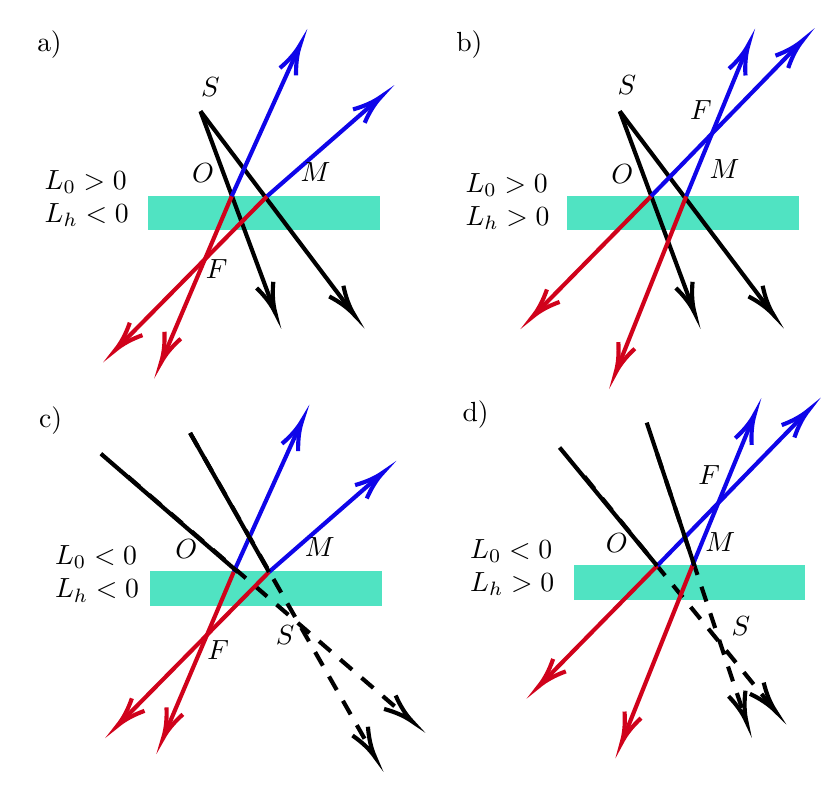
\begin{tikzpicture}[x=0.75pt,y=0.75pt,yscale=-1,xscale=1]
%uncomment if require: \path (0,370); %set diagram left start at 0, and has height of 370

%Shape: Rectangle [id:dp11132417261061733] 
\draw  [color={rgb, 255:red, 80; green, 227; blue, 194 }  ,draw opacity=1 ][fill={rgb, 255:red, 80; green, 227; blue, 194 }  ,fill opacity=1 ] (202,84) -- (313,84) -- (313,100) -- (202,100) -- cycle ;
%Straight Lines [id:da575301150571319] 
\draw [line width=1.5]    (227,43) -- (261.96,137.19) ;
\draw [shift={(263,140)}, rotate = 249.64] [color={rgb, 255:red, 0; green, 0; blue, 0 }  ][line width=1.5]    (14.21,-4.28) .. controls (9.04,-1.82) and (4.3,-0.39) .. (0,0) .. controls (4.3,0.39) and (9.04,1.82) .. (14.21,4.28)   ;
%Straight Lines [id:da14009415856676544] 
\draw [line width=1.5]    (227,43) -- (299.19,138.61) ;
\draw [shift={(301,141)}, rotate = 232.94] [color={rgb, 255:red, 0; green, 0; blue, 0 }  ][line width=1.5]    (14.21,-4.28) .. controls (9.04,-1.82) and (4.3,-0.39) .. (0,0) .. controls (4.3,0.39) and (9.04,1.82) .. (14.21,4.28)   ;
%Straight Lines [id:da7996585837315047] 
\draw [color={rgb, 255:red, 15; green, 5; blue, 233 }  ,draw opacity=1 ][line width=1.5]    (242,84) -- (273.76,13.73) ;
\draw [shift={(275,11)}, rotate = 474.33] [color={rgb, 255:red, 15; green, 5; blue, 233 }  ,draw opacity=1 ][line width=1.5]    (14.21,-4.28) .. controls (9.04,-1.82) and (4.3,-0.39) .. (0,0) .. controls (4.3,0.39) and (9.04,1.82) .. (14.21,4.28)   ;
%Straight Lines [id:da08369442419602358] 
\draw [color={rgb, 255:red, 15; green, 5; blue, 233 }  ,draw opacity=1 ][line width=1.5]    (259,84) -- (311.74,37.97) ;
\draw [shift={(314,36)}, rotate = 498.89] [color={rgb, 255:red, 15; green, 5; blue, 233 }  ,draw opacity=1 ][line width=1.5]    (14.21,-4.28) .. controls (9.04,-1.82) and (4.3,-0.39) .. (0,0) .. controls (4.3,0.39) and (9.04,1.82) .. (14.21,4.28)   ;
%Straight Lines [id:da3206412001442587] 
\draw [color={rgb, 255:red, 208; green, 2; blue, 27 }  ,draw opacity=1 ][line width=1.5]    (259,84) -- (188.11,155.86) ;
\draw [shift={(186,158)}, rotate = 314.61] [color={rgb, 255:red, 208; green, 2; blue, 27 }  ,draw opacity=1 ][line width=1.5]    (14.21,-4.28) .. controls (9.04,-1.82) and (4.3,-0.39) .. (0,0) .. controls (4.3,0.39) and (9.04,1.82) .. (14.21,4.28)   ;
%Straight Lines [id:da8549502068613235] 
\draw [color={rgb, 255:red, 208; green, 2; blue, 27 }  ,draw opacity=1 ][line width=1.5]    (242,84) -- (209.17,161.24) ;
\draw [shift={(208,164)}, rotate = 293.03] [color={rgb, 255:red, 208; green, 2; blue, 27 }  ,draw opacity=1 ][line width=1.5]    (14.21,-4.28) .. controls (9.04,-1.82) and (4.3,-0.39) .. (0,0) .. controls (4.3,0.39) and (9.04,1.82) .. (14.21,4.28)   ;
%Shape: Rectangle [id:dp7208008023108876] 
\draw  [color={rgb, 255:red, 80; green, 227; blue, 194 }  ,draw opacity=1 ][fill={rgb, 255:red, 80; green, 227; blue, 194 }  ,fill opacity=1 ] (404,84) -- (515,84) -- (515,100) -- (404,100) -- cycle ;
%Straight Lines [id:da11626528400135516] 
\draw [line width=1.5]    (429,43) -- (463.96,137.19) ;
\draw [shift={(465,140)}, rotate = 249.64] [color={rgb, 255:red, 0; green, 0; blue, 0 }  ][line width=1.5]    (14.21,-4.28) .. controls (9.04,-1.82) and (4.3,-0.39) .. (0,0) .. controls (4.3,0.39) and (9.04,1.82) .. (14.21,4.28)   ;
%Straight Lines [id:da18225092249170927] 
\draw [line width=1.5]    (429,43) -- (501.19,138.61) ;
\draw [shift={(503,141)}, rotate = 232.94] [color={rgb, 255:red, 0; green, 0; blue, 0 }  ][line width=1.5]    (14.21,-4.28) .. controls (9.04,-1.82) and (4.3,-0.39) .. (0,0) .. controls (4.3,0.39) and (9.04,1.82) .. (14.21,4.28)   ;
%Straight Lines [id:da23120296389327732] 
\draw [color={rgb, 255:red, 15; green, 5; blue, 233 }  ,draw opacity=1 ][line width=1.5]    (444,84) -- (514.91,11.15) ;
\draw [shift={(517,9)}, rotate = 494.23] [color={rgb, 255:red, 15; green, 5; blue, 233 }  ,draw opacity=1 ][line width=1.5]    (14.21,-4.28) .. controls (9.04,-1.82) and (4.3,-0.39) .. (0,0) .. controls (4.3,0.39) and (9.04,1.82) .. (14.21,4.28)   ;
%Straight Lines [id:da7232424824933374] 
\draw [color={rgb, 255:red, 15; green, 5; blue, 233 }  ,draw opacity=1 ][line width=1.5]    (461,84) -- (489.86,13.77) ;
\draw [shift={(491,11)}, rotate = 472.34] [color={rgb, 255:red, 15; green, 5; blue, 233 }  ,draw opacity=1 ][line width=1.5]    (14.21,-4.28) .. controls (9.04,-1.82) and (4.3,-0.39) .. (0,0) .. controls (4.3,0.39) and (9.04,1.82) .. (14.21,4.28)   ;
%Straight Lines [id:da39109169227709817] 
\draw [color={rgb, 255:red, 208; green, 2; blue, 27 }  ,draw opacity=1 ][line width=1.5]    (461,84) -- (428.11,166.21) ;
\draw [shift={(427,169)}, rotate = 291.8] [color={rgb, 255:red, 208; green, 2; blue, 27 }  ,draw opacity=1 ][line width=1.5]    (14.21,-4.28) .. controls (9.04,-1.82) and (4.3,-0.39) .. (0,0) .. controls (4.3,0.39) and (9.04,1.82) .. (14.21,4.28)   ;
%Straight Lines [id:da07625434489085259] 
\draw [color={rgb, 255:red, 208; green, 2; blue, 27 }  ,draw opacity=1 ][line width=1.5]    (444,84) -- (389.1,139.86) ;
\draw [shift={(387,142)}, rotate = 314.5] [color={rgb, 255:red, 208; green, 2; blue, 27 }  ,draw opacity=1 ][line width=1.5]    (14.21,-4.28) .. controls (9.04,-1.82) and (4.3,-0.39) .. (0,0) .. controls (4.3,0.39) and (9.04,1.82) .. (14.21,4.28)   ;
%Shape: Rectangle [id:dp6635565575130467] 
\draw  [color={rgb, 255:red, 80; green, 227; blue, 194 }  ,draw opacity=1 ][fill={rgb, 255:red, 80; green, 227; blue, 194 }  ,fill opacity=1 ] (203,265) -- (314,265) -- (314,281) -- (203,281) -- cycle ;
%Straight Lines [id:da610645942337422] 
\draw [line width=1.5]  [dash pattern={on 5.63pt off 4.5pt}]  (192,219) -- (326.73,335.04) ;
\draw [shift={(329,337)}, rotate = 220.74] [color={rgb, 255:red, 0; green, 0; blue, 0 }  ][line width=1.5]    (14.21,-4.28) .. controls (9.04,-1.82) and (4.3,-0.39) .. (0,0) .. controls (4.3,0.39) and (9.04,1.82) .. (14.21,4.28)   ;
%Straight Lines [id:da7904642819600727] 
\draw [line width=1.5]  [dash pattern={on 5.63pt off 4.5pt}]  (222,198) -- (309.51,351.39) ;
\draw [shift={(311,354)}, rotate = 240.29] [color={rgb, 255:red, 0; green, 0; blue, 0 }  ][line width=1.5]    (14.21,-4.28) .. controls (9.04,-1.82) and (4.3,-0.39) .. (0,0) .. controls (4.3,0.39) and (9.04,1.82) .. (14.21,4.28)   ;
%Straight Lines [id:da9517710980434895] 
\draw [color={rgb, 255:red, 15; green, 5; blue, 233 }  ,draw opacity=1 ][line width=1.5]    (243,265) -- (274.76,194.73) ;
\draw [shift={(276,192)}, rotate = 474.33] [color={rgb, 255:red, 15; green, 5; blue, 233 }  ,draw opacity=1 ][line width=1.5]    (14.21,-4.28) .. controls (9.04,-1.82) and (4.3,-0.39) .. (0,0) .. controls (4.3,0.39) and (9.04,1.82) .. (14.21,4.28)   ;
%Straight Lines [id:da04530062637847765] 
\draw [color={rgb, 255:red, 15; green, 5; blue, 233 }  ,draw opacity=1 ][line width=1.5]    (260,265) -- (312.74,218.97) ;
\draw [shift={(315,217)}, rotate = 498.89] [color={rgb, 255:red, 15; green, 5; blue, 233 }  ,draw opacity=1 ][line width=1.5]    (14.21,-4.28) .. controls (9.04,-1.82) and (4.3,-0.39) .. (0,0) .. controls (4.3,0.39) and (9.04,1.82) .. (14.21,4.28)   ;
%Straight Lines [id:da6878902056022982] 
\draw [color={rgb, 255:red, 208; green, 2; blue, 27 }  ,draw opacity=1 ][line width=1.5]    (260,265) -- (189.11,336.86) ;
\draw [shift={(187,339)}, rotate = 314.61] [color={rgb, 255:red, 208; green, 2; blue, 27 }  ,draw opacity=1 ][line width=1.5]    (14.21,-4.28) .. controls (9.04,-1.82) and (4.3,-0.39) .. (0,0) .. controls (4.3,0.39) and (9.04,1.82) .. (14.21,4.28)   ;
%Straight Lines [id:da7782177313790433] 
\draw [color={rgb, 255:red, 208; green, 2; blue, 27 }  ,draw opacity=1 ][line width=1.5]    (243,265) -- (210.17,342.24) ;
\draw [shift={(209,345)}, rotate = 293.03] [color={rgb, 255:red, 208; green, 2; blue, 27 }  ,draw opacity=1 ][line width=1.5]    (14.21,-4.28) .. controls (9.04,-1.82) and (4.3,-0.39) .. (0,0) .. controls (4.3,0.39) and (9.04,1.82) .. (14.21,4.28)   ;
%Shape: Rectangle [id:dp1905344005637597] 
\draw  [color={rgb, 255:red, 80; green, 227; blue, 194 }  ,draw opacity=1 ][fill={rgb, 255:red, 80; green, 227; blue, 194 }  ,fill opacity=1 ] (407,262) -- (518,262) -- (518,278) -- (407,278) -- cycle ;
%Straight Lines [id:da7837054554442535] 
\draw [line width=1.5]  [dash pattern={on 5.63pt off 4.5pt}]  (412,219) -- (502.11,329.67) ;
\draw [shift={(504,332)}, rotate = 230.85] [color={rgb, 255:red, 0; green, 0; blue, 0 }  ][line width=1.5]    (14.21,-4.28) .. controls (9.04,-1.82) and (4.3,-0.39) .. (0,0) .. controls (4.3,0.39) and (9.04,1.82) .. (14.21,4.28)   ;
%Straight Lines [id:da6951316937673788] 
\draw [line width=1.5]  [dash pattern={on 5.63pt off 4.5pt}]  (447,208) -- (489.05,334.15) ;
\draw [shift={(490,337)}, rotate = 251.57] [color={rgb, 255:red, 0; green, 0; blue, 0 }  ][line width=1.5]    (14.21,-4.28) .. controls (9.04,-1.82) and (4.3,-0.39) .. (0,0) .. controls (4.3,0.39) and (9.04,1.82) .. (14.21,4.28)   ;
%Straight Lines [id:da3602109129464701] 
\draw [color={rgb, 255:red, 15; green, 5; blue, 233 }  ,draw opacity=1 ][line width=1.5]    (447,262) -- (517.91,189.15) ;
\draw [shift={(520,187)}, rotate = 494.23] [color={rgb, 255:red, 15; green, 5; blue, 233 }  ,draw opacity=1 ][line width=1.5]    (14.21,-4.28) .. controls (9.04,-1.82) and (4.3,-0.39) .. (0,0) .. controls (4.3,0.39) and (9.04,1.82) .. (14.21,4.28)   ;
%Straight Lines [id:da5387934912810612] 
\draw [color={rgb, 255:red, 15; green, 5; blue, 233 }  ,draw opacity=1 ][line width=1.5]    (464,262) -- (492.86,191.77) ;
\draw [shift={(494,189)}, rotate = 472.34] [color={rgb, 255:red, 15; green, 5; blue, 233 }  ,draw opacity=1 ][line width=1.5]    (14.21,-4.28) .. controls (9.04,-1.82) and (4.3,-0.39) .. (0,0) .. controls (4.3,0.39) and (9.04,1.82) .. (14.21,4.28)   ;
%Straight Lines [id:da040960058403754385] 
\draw [color={rgb, 255:red, 208; green, 2; blue, 27 }  ,draw opacity=1 ][line width=1.5]    (464,262) -- (431.11,344.21) ;
\draw [shift={(430,347)}, rotate = 291.8] [color={rgb, 255:red, 208; green, 2; blue, 27 }  ,draw opacity=1 ][line width=1.5]    (14.21,-4.28) .. controls (9.04,-1.82) and (4.3,-0.39) .. (0,0) .. controls (4.3,0.39) and (9.04,1.82) .. (14.21,4.28)   ;
%Straight Lines [id:da47493755539430027] 
\draw [color={rgb, 255:red, 208; green, 2; blue, 27 }  ,draw opacity=1 ][line width=1.5]    (447,262) -- (392.1,317.86) ;
\draw [shift={(390,320)}, rotate = 314.5] [color={rgb, 255:red, 208; green, 2; blue, 27 }  ,draw opacity=1 ][line width=1.5]    (14.21,-4.28) .. controls (9.04,-1.82) and (4.3,-0.39) .. (0,0) .. controls (4.3,0.39) and (9.04,1.82) .. (14.21,4.28)   ;
%Straight Lines [id:da5951211705904946] 
\draw [line width=1.5]    (442,193) -- (465,262) ;
%Straight Lines [id:da4840835275161879] 
\draw [line width=1.5]    (400,205) -- (447,262) ;
%Straight Lines [id:da7227713867888061] 
\draw [line width=1.5]    (222,198) -- (260,265) ;
%Straight Lines [id:da17973503463946772] 
\draw [line width=1.5]    (179,208) -- (245,265) ;

% Text Node
\draw (221.67,67) node [anchor=north west][inner sep=0.75pt]   [align=left] {$\displaystyle O$};
% Text Node
\draw (274,66.67) node [anchor=north west][inner sep=0.75pt]   [align=left] {$\displaystyle M$};
% Text Node
\draw (226,25.67) node [anchor=north west][inner sep=0.75pt]   [align=left] {$\displaystyle S$};
% Text Node
\draw (144,68) node [anchor=north west][inner sep=0.75pt]   [align=left] {$\displaystyle  \begin{array}{{>{\displaystyle}l}}
L_{0}  >0\\
L_{h} < 0
\end{array}$};
% Text Node
\draw (228.33,113.33) node [anchor=north west][inner sep=0.75pt]   [align=left] {$\displaystyle F$};
% Text Node
\draw (147,3) node [anchor=north west][inner sep=0.75pt]   [align=left] {a)};
% Text Node
\draw (423.67,67.33) node [anchor=north west][inner sep=0.75pt]   [align=left] {$\displaystyle O$};
% Text Node
\draw (471,65) node [anchor=north west][inner sep=0.75pt]   [align=left] {$\displaystyle M$};
% Text Node
\draw (426.67,24.67) node [anchor=north west][inner sep=0.75pt]   [align=left] {$\displaystyle S$};
% Text Node
\draw (346.8,69.6) node [anchor=north west][inner sep=0.75pt]   [align=left] {$\displaystyle  \begin{array}{{>{\displaystyle}l}}
L_{0}  >0\\
L_{h}  >0
\end{array}$};
% Text Node
\draw (461.67,36.67) node [anchor=north west][inner sep=0.75pt]   [align=left] {$\displaystyle F$};
% Text Node
\draw (349,3) node [anchor=north west][inner sep=0.75pt]   [align=left] {b)};
% Text Node
\draw (213.67,248.33) node [anchor=north west][inner sep=0.75pt]   [align=left] {$\displaystyle O$};
% Text Node
\draw (276,247) node [anchor=north west][inner sep=0.75pt]   [align=left] {$\displaystyle M$};
% Text Node
\draw (262,289.67) node [anchor=north west][inner sep=0.75pt]   [align=left] {$\displaystyle S$};
% Text Node
\draw (149,249) node [anchor=north west][inner sep=0.75pt]   [align=left] {$\displaystyle  \begin{array}{{>{\displaystyle}l}}
L_{0} < 0\\
L_{h} < 0
\end{array}$};
% Text Node
\draw (229,297) node [anchor=north west][inner sep=0.75pt]   [align=left] {$\displaystyle F$};
% Text Node
\draw (148,184) node [anchor=north west][inner sep=0.75pt]   [align=left] {c)};
% Text Node
\draw (421,245) node [anchor=north west][inner sep=0.75pt]   [align=left] {$\displaystyle O$};
% Text Node
\draw (469,244.67) node [anchor=north west][inner sep=0.75pt]   [align=left] {$\displaystyle M$};
% Text Node
\draw (481.67,285.33) node [anchor=north west][inner sep=0.75pt]   [align=left] {$\displaystyle S$};
% Text Node
\draw (349,246) node [anchor=north west][inner sep=0.75pt]   [align=left] {$\displaystyle  \begin{array}{{>{\displaystyle}l}}
L_{0} < 0\\
L_{h}  >0
\end{array}$};
% Text Node
\draw (465.67,212.33) node [anchor=north west][inner sep=0.75pt]   [align=left] {$\displaystyle F$};
% Text Node
\draw (352,181) node [anchor=north west][inner sep=0.75pt]   [align=left] {d)};


\end{tikzpicture}



\end{figure}

%%%%%%%%%%%%%%%%%%%%%%%%%%%%%%%%  end put here figure %%%%%%%%%%%%%%%%%%%%%%%%%%%%%%%%%%%%%%%%%%%%%%%%

\end{document}